% !TeX program = lualatex
% !TeX encoding = utf8
% !TeX spellcheck = uk_UA
% !BIB program = bibler

\documentclass[9pt]{beamer}
\usetheme{Electromagnetism}
\usepackage{Electromagnetism}
\usepackage{physics}
\usepackage{tikz}
\usepackage{tikz-3dplot}
\usepackage[outline]{contour} % glow around text
\usepackage{xcolor}
\tikzset{cone/.pic = {
             \draw (-0.5, 0.5) coordinate (-nw) -- ++ (1,-1) coordinate (-se);
             \draw (-0.5,-0.5) coordinate (-sw) -- ++ (1, 1) coordinate (-ne);
             \fill (0,0)  coordinate (-center) circle (0.05);
             \draw (0, 0.5) ellipse (0.5 and 0.05);
             \draw (0,-0.5) ellipse (0.5 and 0.05);
             \coordinate (-top)     at (0, 0.55);
             \coordinate (-north)   at (0, 0.5);
             \coordinate (-south)   at (0,-0.5);
             \coordinate (-bottom)  at (0,-0.55);
            }
            }
\tikzset{middlearrow/.style={
        decoration={markings,
            mark= at position 0.5 with {\arrow{#1}} ,
        },
        postaction={decorate}
    }
}
\newtcolorbox{pict}{
colback=white,
colframe=gray,
boxrule=0.1pt,
left=0pt,
right=0pt,
top=0pt,
bottom=0pt,
sharp corners,
halign=center,
enhanced,drop fuzzy shadow,
hbox,
}

\let\vect\vec
%============================================================================
\title[]{\huge\bfseries  Міні-лабораторія з Arduino}
\date{}
%============================================================================
\graphicspath{{pictures/}}

%\addtobeamertemplate{frametitle}{}{%
%\begin{tikzpicture}[remember picture,overlay]
%\node[anchor=north west] at (current page.north west) {\includegraphics[height=1cm]{logo}};
%\end{tikzpicture}}


%\titlegraphic{\includegraphics[width=0.25\linewidth]{Einstein}}

\begin{document}
\begin{frame}[plain]
	\tikz [remember picture,overlay]
	\node[anchor=south west, opacity=0.9] at
	(current page.south west)
	%or: (current page.center)
	{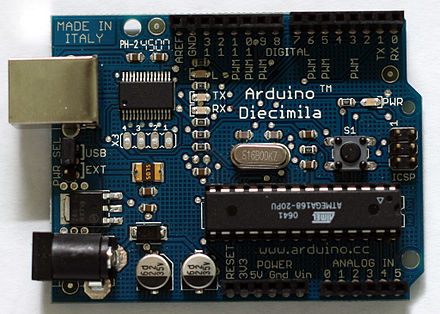
\includegraphics[width=0.25\linewidth]{pictures/arduino}};
	\maketitle
\end{frame}

% ============================== Слайд ## ===================================
\begin{frame}{Що таке Arduino?}{}
       \begin{block}{}\justifying
       Arduino --- це компактна електронна плата, здатна керувати різними датчиками, електродвигунами, індикацією, освітленням, передавати та приймати дані безпосередньо на компьютер.
       \end{block}

       \begin{center}
           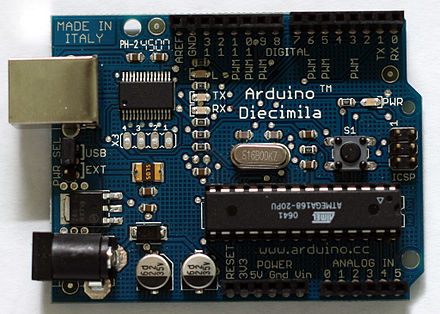
\includegraphics[width=0.5\linewidth]{pictures/arduino}
       \end{center}
\end{frame}
% ===========================================================================

% ============================== Слайд ## ===================================
\begin{frame}{Як взаємодіє Arduino із зовнішнім світом?}{}
     \begin{block}{}
     Щоб Arduino міг взаємодіяти із зовнішнім світом, у нього є вхідні/вихідні піни (контакт), які розміщені по периметру плати.
     \end{block}

            \begin{center}
                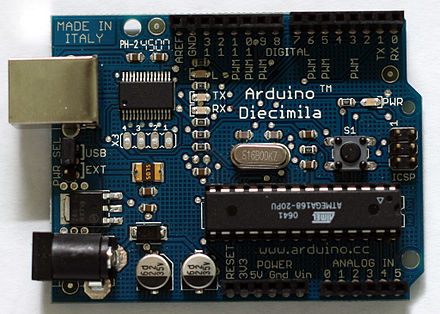
\includegraphics[width=0.5\linewidth]{pictures/arduino}
            \end{center}
\end{frame}
% ===========================================================================

% ============================== Слайд ## ===================================
\begin{frame}{Чим може керувати Arduino?}{}
\begin{columns}
	\begin{column}{0.5\linewidth}
         \begin{block}{}
         Ось перелік найпопулярніших варіантів:

         \begin{itemize}
         \item датчики температури, вологості, освітленості, руху та ін;
         \item РК дисплеї, індикатори, світлодіоди;
         \item зчитувачі SD-карт;
         \item GPS і GSM модулі;
         \item і багато іншого.
         \end{itemize}
         \end{block}
	\end{column}
	\begin{column}{0.5\linewidth}
             \begin{center}
                 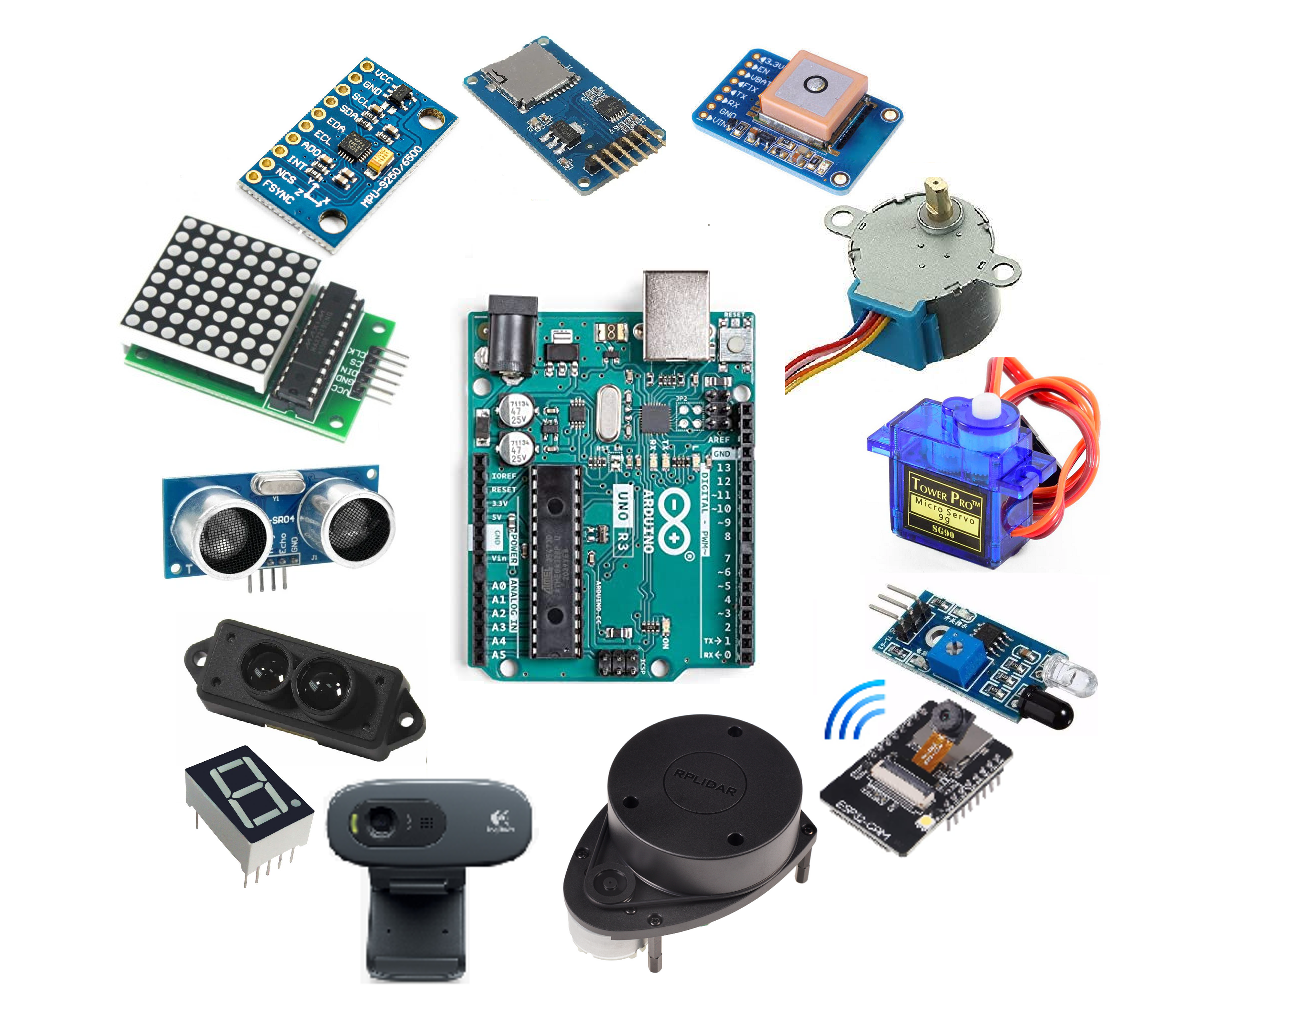
\includegraphics[width=\linewidth]{pictures/arduino_sensors}
             \end{center}
	\end{column}
\end{columns}


\end{frame}
% ===========================================================================

% ============================== Слайд ## ===================================
\begin{frame}{Домашня лабораторія з Arduino}{}
       \begin{block}{}
       Завдяки <<всеїдності>> Arduino можна перетворити на домашню лабораторію.
       \end{block}
    \begin{center}
        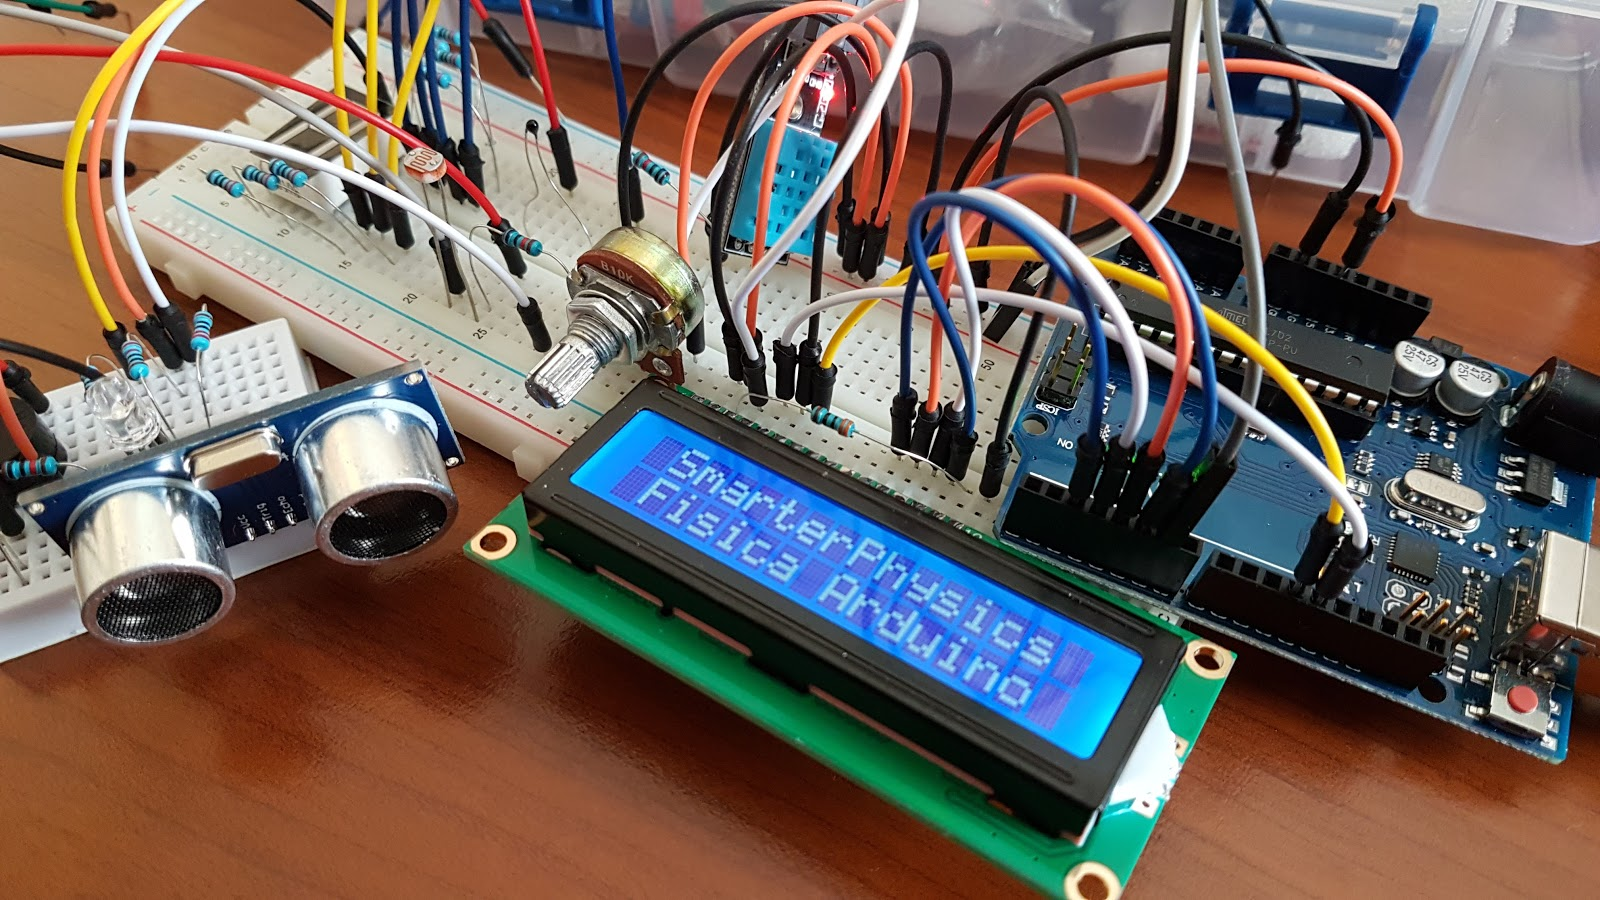
\includegraphics[width=\linewidth]{pictures/arduino_physics}
    \end{center}
\end{frame}
% ===========================================================================

% ============================== Слайд ## ===================================
\begin{frame}{Вимірювання температури}{}
\textbf{Термопара}: \texttt{Термопара K-типу з цифровим підсилювачес на чіпі MAX6675. Систематична абсолютна похибка термопари: $\pm 0.25^\circ$C}

\begin{columns}
	\begin{column}{0.5\linewidth}
         \begin{tikzpicture}[scale=0.9]
             \begin{axis}[%
             title={Heating time domain},
             width=0.85\linewidth,
             height=0.75\linewidth,
             			xlabel={$t$ / min},
             			ylabel={$T$ / ${^\circ}$C},
             scale only axis,
             enlargelimits=false,
             line join=round,
             % === Налаштування сітки ===
             grid = both,
             grid style={line width=.1pt, draw=gray!10},
             major grid style={line width=.2pt,draw=gray!50},
             minor tick num = 5,
             minor grid style = {line width=.1pt,draw=gray!10},
             xmin=6,
             xmax=10,
             ymax=55
             ]
             \addplot [color=red, line width=1pt, mark=*, mark size=1pt] table [x expr=\coordindex * 1 / 60, y=y] {data.txt};

         %    \addplot[domain=0:45, blue, ultra thick] {25 + (90  - 25)*exp(-0.045*x^0.94)};
             \node[anchor=south east,
             		draw=none,
             		fill=white,
                     font=\ttfamily\small,
             		align=left,
             		fill opacity=0.5,
             		text opacity=1,
             		] at ([shift ={(0cm,1cm)}]current axis.south east) {
         %    		Room temperature: $T_0 = 23^\circ$C\\
         %            Systematic absolute error of the sensor: $\pm 0.25^\circ$C
                     };

             \end{axis}

             \end{tikzpicture}
	\end{column}
	\begin{column}{0.5\linewidth}
 \begin{tikzpicture}[scale=0.9]
     \begin{axis}[%
     title={Cooling time domain},
     width=0.85\linewidth,
     height=0.75\linewidth,
     			xlabel={$t$ / min},
     			ylabel={$T$ / ${^\circ}$C},
     scale only axis,
     enlargelimits=false,
     line join=round,
     % === Налаштування сітки ===
     grid = both,
     grid style={line width=.1pt, draw=gray!10},
     major grid style={line width=.2pt,draw=gray!50},
     minor tick num = 5,
     minor grid style = {line width=.1pt,draw=gray!10},
     xmin=10,
     ymin=23,
     ymax=55
     ]
     \addplot [color=red, line width=1pt, mark=*, mark size=1pt] table [x expr=\coordindex * 1 / 60, y=y] {data.txt};

 %    \addplot[domain=0:45, blue, ultra thick] {25 + (90  - 25)*exp(-0.045*x^0.94)};
     \node[anchor=south east,
     		draw=none,
     		fill=white,
             font=\ttfamily\small,
     		align=left,
     		fill opacity=0.5,
     		text opacity=1,
     		] at ([shift ={(0cm,1cm)}]current axis.south east) {
 %    		Room temperature: $T_0 = 23^\circ$C\\
 %            Systematic absolute error of the sensor: $\pm 0.25^\circ$C
             };

     \end{axis}

     \end{tikzpicture}
	\end{column}
\end{columns}

\end{frame}
% ===========================================================================

\end{document}
